\documentclass[a4paper,10pt]{article}
\usepackage{graphicx}
\usepackage{amsmath}
\usepackage{amssymb}
\usepackage[italian]{babel}
\usepackage[T1]{fontenc}
\usepackage[utf8]{inputenc}
\usepackage[margin=1.25in]{geometry}

\usepackage[backend=biber]{biblatex}
\addbibresource{ref.bib}

\begin{document}

   \title{{\large Universita' degli Studi di Padova \\ } {\normalsize Corso di laurea triennale in Ingegneria Informatica}\\ \vspace{1.8cm} \textbf{ Homework 2: Strumenti per la valutazione delle prestazioni di rete}}
   
   \author{Giacomo Camposampiero, matricola 1187180} 
   \date{20 novembre 2020}
   \maketitle
   \vspace{2.2cm}
   \renewcommand{\contentsname}{Indice}      
   \tableofcontents
   \newpage

\section{Comando \texttt{ping} }
\texttt{ping} (Packet INternet Groper) è un software di amministrazione per reti di computer utilizzato per verificare la raggiungibilità di un host all'interno di una rete IP. Questa applicazione è supportata nella maggior parte dei sistemi operativi comuni ed è ampiamente utilizzata come strumento elementare di diagnostica di rete. 

Il funzionamento di \texttt{ping} è interamente basato sul protocollo ICMP (Internet Control Message Protocol, RFC 792), che si appoggia direttamente ai servizi offerti dall'Internet Protocol, senza coinvolgere alcun tipo di servizio di livello di trasporto. L'applicazione invia una serie di pacchetti \texttt{ICMP Echo Request} ad una destinazione, la quale risponde ad ogni pacchetto ricevuto inviando un corrispettivo pacchetto \texttt{ICMP Echo Reply} di risposta della stessa dimensione della richiesta. Una rappresentazione grafica della struttura di un pacchetto ICMP è riportata in Figura \ref{fig:ICMP}. \texttt{ping} misura il cosiddetto \textit{Round-Trip Time} (RTT), ovvero il tempo che intercorre tra l'invio della richiesta e la ricezione della risposta, per poi visualizzarlo in output.

\begin{figure}[h!]
	\centering
	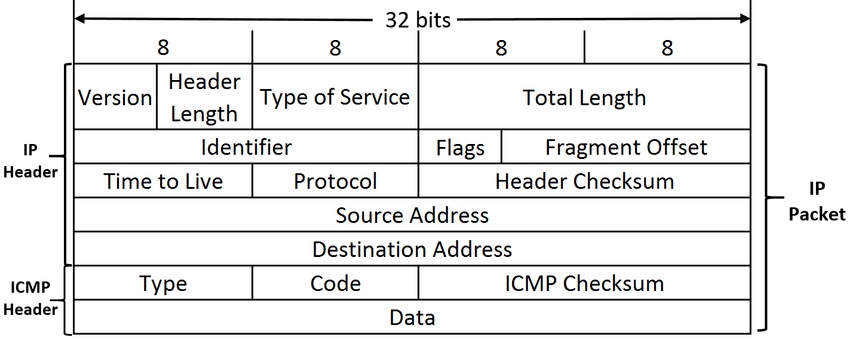
\includegraphics[scale=0.25]{img/icmp.png}
  	\caption{Struttura pacchetto ICMP \cite{ref:icmp}}
  	\label{fig:ICMP}
\end{figure}


\subsection{Opzioni}
Il software \texttt{ping} offre numerose opzioni da linea di comando, che possono variare a seconda del sistema operativo in cui è implementato e dei privilegi posseduti dall'utente che lo invoca. Una lista delle opzioni disponibili può essere ottenuta dall'utente mediante l'invocazione del comando \texttt{man ping}. Di seguito è riportato un elenco delle opzioni che sono state giudicate più utili nella valutazione delle prestazioni di una connessione.
\begin{itemize}
\item Prova
\end{itemize}
Al fine di definire il numero \textit{C} di pacchetti ICMP ECHO REQUEST inviati per ogni sessione, è presente nel programma la seguente opzione.
\begin{quote}
\begin{verbatim}
-c count
	Stop after sending count ECHO_REQUEST packets. With deadline option, ping 
	waits for count ECHO_REPLY packets, until the timeout expires.
\end{verbatim}
\end{quote}  

\newpage

\printbibliography

\newpage

\subsection{RTT}
RTT corrisponde alla somma dei ritardi accumulati nel percorso di andata (tra sorgente e destinazione) e di ritorno (viceversa). Numerando da 1 a \textit{n} i nodi attraversati durante l'intero tragitto comprensivo di andata e ritorno, il RTT del \textit{k}-esimo scambio request-reply si calcola come
\begin{align*}
RTT(k) = \sum_{i=1}^{n} \left( \frac{L(k)}{R_i} + q_i(k) + \tau_i \right)
\end{align*}
dove
\begin{itemize}
\item $L(k)$ è la dimensione a livello rete (IP) della PDU che trasporta i pacchetti Request/Reply delkesimo ciclo.  Detta $l(k)$ la lunghezza del payload del pacchetto ICMP Echo Request/Reply, e considerando che il protocollo ICMP aggiunge 8 byte di header, e il protocollo IP altri 20 byte di header, si haL(k) =`(k) + 28×8[bit] a livello IP.
\item $R_i$ è il bitrate offerto dal link \textit{i}-esimo a livello rete (ovvero, il throughput visto del protocollo di rete IP) in bit/s.
\item $q_i(k)$ è il tempo speso dal pacchetto nel buffer di trasmissione del link \textit{i}-esimo.
\item $\tau_i$ è il tempo di propagazione lungo il link \textit{i}-esimo.
\end{itemize}

\subsection{Simulare il diagramma di Bode dell'ampiezza tra 1Hz e 100 kHz}
Per simulare il diagramma di Bode dell'ampiezza e' stato utilizzato il listato SPICE riportato di seguito. Il risultato dell'analisi in frequenza e' riportato graficamente (Figure \ref{fig:bode1}).
\begin{quote}
\begin{verbatim}
* Esercizio 1.3
Vin N1 0 DC 0 AC 1 sin(0 10mV 10kHz 0 0 0)
VDD N2 0 10V
VSS N3 0 -10V
XU1 Vp Vn N2 N3 Vo LT1028
C2 Vp N1 100n
R2 Vp 0 100k
R4 Vn Vo 10k
R3 Vn 0 1k
.lib LTC.lib
.ac DEC 10 1 100k
.backanno
.end
\end{verbatim}
\end{quote}


\subsection{Per quale ampiezza del segnale di ingresso l'uscita satura? Simulare la forma  d'onda di uscita per un segnale di ingresso di ampiezza pari a 2 volte il valore trovato}
Innanzitutto, troviamo sperimentalmente l'ampiezza a cui satura l'amplificatore operazionale, fornendo al circuito segnali di svariate ampiezze e medesima frequenza (10kHz) in ingresso. Per fare cio', parametrizziamo l'ampiezza del segnale in ingresso e la facciamo variare a step di 200mV tra 100mV e 3V.
\small
\begin{quote}
\begin{verbatim}
* Esercizio 1.4
Vin N1 0 DC 0 AC 1 sin(0 {A} 10kHz 0 0 0)
VDD N2 0 10V
VSS N3 0 -10V
XU1 Vp Vn N2 N3 Vo LT1028
C2 Vp N1 100n
R2 Vp 0 100k
R4 Vn Vo 10k
R3 Vn 0 1k
.lib LTC.lib
.tran 0 0.5m
.step param A 100m 3 200m
.backanno
.end
\end{verbatim}
\end{quote}
\normalsize
\begin{figure}[h!]
	\centering
  	\caption{Forma d'onda in uscita al variare dell'ampiezza in ingresso.}
  	\label{fig:sat1}
\end{figure}
Dai risultati sperimentali si puo' dedurre che l'amplificatore satura ad un'ampiezza all'incirca pari a $8$V (se fosse ideale saturerebbe ad un'ampiezza in modulo di $10$V, ovvero la tensione di alimentazione in modulo fornita all'amplificatore operazionale). Troviamo analiticamente l'ampiezza del segnale in ingresso per cui appare il fenomeno di distorsione.
\begin{gather*}
	\lvert V_o \rvert\ = \lvert W(j\omega) \rvert\ \cdot \lvert V_{in} \rvert\ = \lvert \frac{2200j\pi}{1+200j\pi} \rvert\ \cdot \lvert V_{in} \rvert\ \\
	\Rightarrow \lvert V_{in} \rvert\ = \frac{8\cdot \sqrt{1+400\pi^2}}{2200\pi} = 0.727\,V
\end{gather*}
La forma d'onda del segnale di uscita, nel caso di un ingresso di ampiezza pari al doppio dell'ampiezza appena calcolata, e' riportata di seguito (Figure \ref{fig:sat2}).
    
\begin{figure}[h!]
	\centering
  	\caption{Forma d'onda in uscita con ingresso di ampiezza 1.45V.}
  	\label{fig:sat2}
\end{figure}

\subsection{Ripetere sostituendo a R2 una resistenza di valore pari al vostro numero di matricola diviso 100}
Sostituendo al valore della resistenza R2 il mio numero di matricola diviso 100 (R2 = 11871.8$\Omega$) i risultati ottenuti nei punti precedenti cambiano di conseguenza. La frequenza di taglio viene ricalcolata di seguito, mentre il guadagno ad altra frequenza rimane invariato in quanto indipendente da R2.
\begin{align*}
\omega_1 = \frac{1}{C_2R_2} = 842.33 \frac{rad}{s} = 134.06Hz
\end{align*}
Per quanto riguarda le nuove forme d'onda in uscita alle diverse frequenze (1Hz, 10Hz e 10kHz), i nuovi grafici sono rappresentati nelle figure Figure \ref{fig:plot1hzr2}, Figure \ref{fig:plot10hzr2} e Figure \ref{fig:plot10khzr2}. Il diagramma di Bode tra le frequenze di 1Hz e 100kHz aggiornato diventa quello rappresentato in figura Figure \ref{fig:plotboder2}.
\begin{figure}[h!]
	\centering
  	\caption{Ingresso a 1Hz con valore di resistenza R2 aggiornato.}
  	\label{fig:plot1hzr2}
\end{figure}

\begin{figure}[h!]
	\centering
  	\caption{Ingresso a 10Hz con valore di resistenza R2 aggiornato.}
  	\label{fig:plot10hzr2}
\end{figure}

\begin{figure}[h!]
	\centering
  	\caption{Ingresso a 10kHz con valore di resistenza R2 aggiornato.}
  	\label{fig:plot10khzr2}
\end{figure}

\begin{figure}[h!]
	\centering
  	\caption{Diagramma di Bode con valore di resistenza R2 aggiornato.}
  	\label{fig:plotboder2}
\end{figure}

\pagebreak
Per quanto riguarda la saturazione, infine, ripetiamo la ricerca sperimentale dell'ampiezza massima a cui satura il segnale in uscita (con lo stesso listato SPICE del punto 1.4, in cui viene sostituito solamente il valore della resistenza R2). Il risultato e' riportato in figura Figure \ref{fig:plotsatr2}.

\begin{figure}[h!]
	\centering
  	\caption{Ricerca sperimentale dell'ampiezza a cui satura l'amplificatore.}
  	\label{fig:plotsatr2}
\end{figure}

Successivamente, ricalcoliamo analiticamente l'ampiezza del segnale in ingresso per cui l'amplificatore satura e riportiamo la forma d'onda del segnale in uscita a fronte di un ingresso di ampiezza doppia rispetto a quella trovata algebricamente.
\begin{align*}
\lvert V_o \rvert\ = \lvert W(j\omega) \rvert\ \cdot \lvert V_{in} \rvert\ \Rightarrow \lvert V_{in} \rvert\ = 0.737\,V
\end{align*}
Il grafico della forma d'onda in uscita a fronte di un segnale in ingresso di ampiezza pari al doppio dell'ampiezza appena calcolata e' riportato di seguito (Figure \ref{fig:plottaglior2}).
\begin{figure}[h!]
	\centering
  	\caption{Forma d'onda del segnale in uscita con ampiezza doppia rispetto a quella calcolata.}
  	\label{fig:plottaglior2}
\end{figure}

\newpage

\subsection{Qual e' la potenza assorbita dall'alimentazione nei due casi?}
La potenza assorbita dall'amplificatore operazionale corrisponde alla somma delle potenze erogate dai due generatori con cui e' alimentato l'amplificatore operazionale stesso. Quest'ultima puo' essere calcolata come
\begin{align*}
P_{out, alimentazione} = V_{ss} \cdot I_{ss} + V_{dd} \cdot I_{dd}
\end{align*}
Misurando questa grandezza, troviamo la potenza erogata dall'alimentazione per i due diversi valori di resistenza R2 100k$\Omega$ e 11871.8$\Omega$ (rispettivamente Figure \ref{fig:pow1} e Figure \ref{fig:pow2}).

\begin{figure}[h!]
	\centering
  	\caption{Resistenza R2 pari a 100k$\Omega$.}
  	\label{fig:pow1}
\end{figure}

\begin{figure}[h!]
	\centering
  	\caption{Resistenza R2 pari a 11\,871.8$\Omega$.}
  	\label{fig:pow2}
\end{figure}

Possiamo notare come non sia visibile (per questi valori di resistenza) una dipendenza evidente della potenza erogata dal valore della resistenza R2. Inoltre, la potenza del grafico e' negativa, in quanto espressa secondo la convenzione degli utilizzatori (potenze minori di 0 equivalgono a potenze erogate).
\end{document}